% ============================================================
%  Perricheno Platform — 20 Mathematical & IP-Protection Figures
%  v2: vivid palette + compile fixes
%  Compile: pdflatex figures_math_ieee.tex  (twice for fillbetween)
% ============================================================
\documentclass{article}
\usepackage[T1]{fontenc}
\usepackage[utf8]{inputenc}
\usepackage{tikz}
\usepackage{pgfplots}
\pgfplotsset{compat=1.18}
\usetikzlibrary{
  arrows.meta, positioning, shapes.geometric, shapes.multipart,
  fit, backgrounds, decorations.pathreplacing, decorations.markings,
  calc, matrix, patterns, pgfplots.fillbetween
}
\usepackage{xcolor}
\usepackage{amsmath,amssymb}
\usepackage{geometry}
\geometry{a4paper, margin=1.6cm}

% ── Vivid palette (matplotlib 2.0 standard cycle) ─────────────────────────
\definecolor{C1}{RGB}{31,119,180}    % blue
\definecolor{C2}{RGB}{255,127,14}    % orange
\definecolor{C3}{RGB}{44,160,44}     % green
\definecolor{C4}{RGB}{214,39,40}     % red
\definecolor{C5}{RGB}{148,103,189}   % purple
\definecolor{C6}{RGB}{23,190,207}    % teal
\definecolor{C7}{RGB}{188,189,34}    % olive
\definecolor{C8}{RGB}{227,119,194}   % pink
% Vivid medium fills (~50% lighter than above)
\definecolor{F1}{RGB}{162,208,245}   % med blue
\definecolor{F2}{RGB}{255,192,120}   % med orange
\definecolor{F3}{RGB}{158,222,158}   % med green
\definecolor{F4}{RGB}{245,158,158}   % med red
\definecolor{F5}{RGB}{207,185,232}   % med purple
\definecolor{F6}{RGB}{148,228,238}   % med teal
\definecolor{F7}{RGB}{232,233,148}   % med olive
% Light backgrounds
\definecolor{L1}{RGB}{220,237,255}   % light blue
\definecolor{L2}{RGB}{255,228,198}   % light orange
\definecolor{L3}{RGB}{212,244,212}   % light green
\definecolor{L4}{RGB}{255,215,215}   % light red
\definecolor{L5}{RGB}{235,226,250}   % light purple
\definecolor{L6}{RGB}{210,246,250}   % light teal
\definecolor{L7}{RGB}{250,250,210}   % light olive
\definecolor{LGr}{RGB}{238,238,238}  % light gray
\definecolor{DG}{RGB}{35,35,35}      % dark text
\definecolor{MG}{RGB}{115,115,115}   % mid gray

% ── pgfplots base style ───────────────────────────────────────────────────
\pgfplotsset{
  PL/.style={
    width=13cm, height=7.5cm,
    axis lines=left, tick align=outside,
    ticklabel style={font=\footnotesize, color=DG},
    label style={font=\small, color=DG},
    title style={font=\small\bfseries, color=DG},
    legend style={font=\scriptsize, draw=DG!40, rounded corners=3pt,
                  fill=white, inner sep=4pt},
    grid=major, grid style={draw=DG!15, thin, dashed},
    line width=1.6pt, mark size=3.8pt,
  }
}

% ── Definition / Theorem boxes ────────────────────────────────────────────
% Usage: \dbox{C1}{F1}{Def N}{Name}{Body}
\newcommand{\dbox}[5]{%
  \begin{tikzpicture}
    \node[draw=#1, line width=2pt, rounded corners=5pt, fill=#2,
          text width=13cm, align=left, inner sep=9pt,
          font=\small] (B)
      {{\bfseries\color{#1}#3} ({\itshape #4}).\ #5};
  \end{tikzpicture}%
}
\newcommand{\tbox}[2]{%
  \begin{tikzpicture}
    \node[draw=C5, line width=2pt, rounded corners=5pt, fill=L5,
          text width=13cm, align=left, inner sep=9pt, font=\small] (B)
      {{\bfseries\color{C5}#1}.\ #2};
  \end{tikzpicture}%
}

\begin{document}

% ╔══════════════════════════════════════════════════════════════════════════╗
% ║  FIG 1 — Formal Pipeline Composition (Category Theory)                  ║
% ╚══════════════════════════════════════════════════════════════════════════╝
\begin{figure}[h!]
\centering
\dbox{C1}{L1}{Definition 1}{Perricheno Pipeline Algebra}{%
  Let $\mathcal{D}$ be the category of document state spaces.
  The generation pipeline is a composition of six functors
  $F_i : \mathcal{D}_{i-1} \to \mathcal{D}_i$, forming the morphism
  $\Pi = F_5 \circ F_4 \circ F_3 \circ F_{2.5} \circ F_2 \circ F_1 :
  \mathcal{D}_0 \to \mathcal{D}_5$,
  where $\mathcal{D}_0 = $ (prompt, settings, uploads) and
  $\mathcal{D}_5 = $ (compiled PDF, BibTeX, warnings).}

\vspace{0.5em}
\begin{tikzpicture}[
  obj/.style={draw=#1, fill=#2, circle, minimum size=1.15cm,
              font=\scriptsize\bfseries, align=center, inner sep=1pt,
              line width=1.5pt},
  mor/.style={-{Stealth[length=8pt,width=6pt]}, line width=1.4pt, draw=#1},
  lbl/.style={font=\scriptsize\itshape, text=DG, above=4pt},
  sub/.style={font=\tiny, text=MG, below=3pt}
]
\node[obj={DG}{LGr}]  (D0)  at (0,0)     {$\mathcal{D}_0$};
\node[obj={C1}{F1}]   (D1)  at (2.3,0)   {$\mathcal{D}_1$};
\node[obj={C2}{F2}]   (D2)  at (4.6,0)   {$\mathcal{D}_2$};
\node[obj={C5}{F5}]   (D25) at (6.9,0)   {$\mathcal{D}_{2.5}$};
\node[obj={C6}{F6}]   (D3)  at (9.2,0)   {$\mathcal{D}_3$};
\node[obj={C3}{F3}]   (D4)  at (11.5,0)  {$\mathcal{D}_4$};
\node[obj={C4}{F4}]   (D5)  at (13.8,0)  {$\mathcal{D}_5$};

\draw[mor={C1}] (D0)--node[lbl]{$F_1$}node[sub]{Plan}(D1);
\draw[mor={C2}] (D1)--node[lbl]{$F_2$}node[sub]{Extract}(D2);
\draw[mor={C5}] (D2)--node[lbl]{$F_{2.5}$}node[sub]{Verify}(D25);
\draw[mor={C6}] (D25)--node[lbl]{$F_3$}node[sub]{Draft}(D3);
\draw[mor={C3}] (D3)--node[lbl]{$F_4$}node[sub]{Assemble}(D4);
\draw[mor={C4}] (D4)--node[lbl]{$F_5$}node[sub]{Validate}(D5);

\draw[mor={C1}, bend right=38]
  (D0) to node[below=10pt, font=\scriptsize\bfseries, text=C1]
    {$\Pi = F_5 \circ F_4 \circ F_3 \circ F_{2.5} \circ F_2 \circ F_1$} (D5);

\node[font=\tiny\itshape, text=MG] at (6.9,-2.0)
  {$F_4$ (Assemble) is fully deterministic — zero LLM calls.};
\end{tikzpicture}
\caption{Pipeline composition as category morphisms (Definition~1). The full
         transformation $\Pi:\mathcal{D}_0\!\to\!\mathcal{D}_5$ is the
         unique identifier of the Perricheno document generation system.}
\label{fig:category}
\end{figure}

% ╔══════════════════════════════════════════════════════════════════════════╗
% ║  FIG 2 — Confidence Gate Probability Distribution                       ║
% ╚══════════════════════════════════════════════════════════════════════════╝
\begin{figure}[h!]
\centering
\dbox{C5}{L5}{Definition 2}{CGRAG Verification Gate}{%
  Let $\mathbf{c}=(c_1,\ldots,c_5)\in[0,10]^5$ be per-question confidence
  scores. The gate $\Gamma:[0,10]^5\!\to\!\{\texttt{enhanced},\texttt{degraded}\}$:
  $\Gamma(\mathbf{c})=\texttt{enhanced}$ iff
  $\bar{c}\geq\tau_c \;\wedge\; |\sigma|\geq\tau_s \;\wedge\; |\kappa|\geq\tau_k$,
  where $\tau_c=7.0,\;\tau_s=100,\;\tau_k=3$, and
  $\bar{c}=\tfrac{1}{5}\sum_{i=1}^5 c_i$.}

\vspace{0.3em}
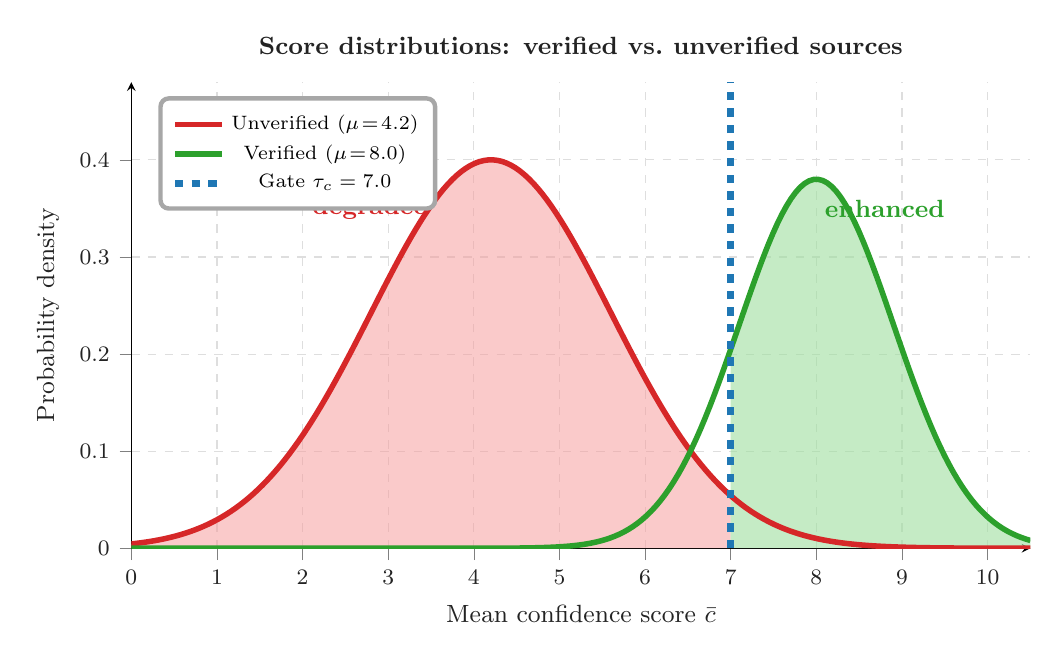
\begin{tikzpicture}
\begin{axis}[PL,
  xlabel={Mean confidence score $\bar{c}$},
  ylabel={Probability density},
  title={Score distributions: verified vs.\ unverified sources},
  xmin=0, xmax=10.5, ymin=0, ymax=0.48,
  xtick={0,1,...,10}, legend pos=north west,
]
% Unverified
\addplot[name path=A, C4, line width=2pt, samples=200, domain=0:10.5]
  {0.40*exp(-((x-4.2)^2)/(2*1.4^2))};
\addlegendentry{Unverified $(\mu\!=\!4.2)$}
% Verified
\addplot[name path=B, C3, line width=2pt, samples=200, domain=0:10.5]
  {0.38*exp(-((x-8.0)^2)/(2*0.9^2))};
\addlegendentry{Verified $(\mu\!=\!8.0)$}
% Threshold
\addplot[name path=T, C1, line width=2.5pt, dashed]
  coordinates{(7.0,0)(7.0,0.48)};
\addlegendentry{Gate $\tau_c=7.0$}
% Fill: unverified region below threshold (bad)
\addplot[name path=ZA, draw=none, domain=0:7.0]{0};
\addplot[F4, opacity=0.55] fill between[of=A and ZA, soft clip={domain=0:7.0}];
% Fill: verified region above threshold (good)
\addplot[name path=ZB, draw=none, domain=7.0:10.5]{0};
\addplot[F3, opacity=0.60] fill between[of=B and ZB, soft clip={domain=7.0:10.5}];
\node[font=\small\bfseries, text=C4] at (axis cs:2.8,0.35) {degraded};
\node[font=\small\bfseries, text=C3] at (axis cs:8.8,0.35) {enhanced};
\end{axis}
\end{tikzpicture}
\caption{Confidence-score distributions for verified vs.\ unverified references.
         Shaded regions mark the accepted/rejected halves of the CGRAG gate
         $\Gamma$ (Definition~2) at threshold $\tau_c\!=\!7.0$.}
\label{fig:cgrag}
\end{figure}

% ╔══════════════════════════════════════════════════════════════════════════╗
% ║  FIG 3 — LCS Dynamic Programming Table                                  ║
% ╚══════════════════════════════════════════════════════════════════════════╝
\begin{figure}[h!]
\centering
\dbox{C3}{L3}{Definition 3}{LCS Label Reconciliation Operator}{%
  Let $\ell_r,\ell_d\in\Sigma^*$ be a \texttt{\textbackslash{}ref} and
  \texttt{\textbackslash{}label} key. The operator
  $\Phi_\theta(\ell_r,\ell_d)$ returns $\ell_d$ iff
  $\mathrm{LCS}(\ell_r,\ell_d)>\theta$, else $\ell_r$, where
  $\mathrm{LCS}(a,b)=\max_{i,j,k}\{k:a[i{:}i{+}k]=b[j{:}j{+}k]\}$
  and $\theta=4$. Complexity: $O(|a|\cdot|b|)$ time.}

\vspace{0.4em}
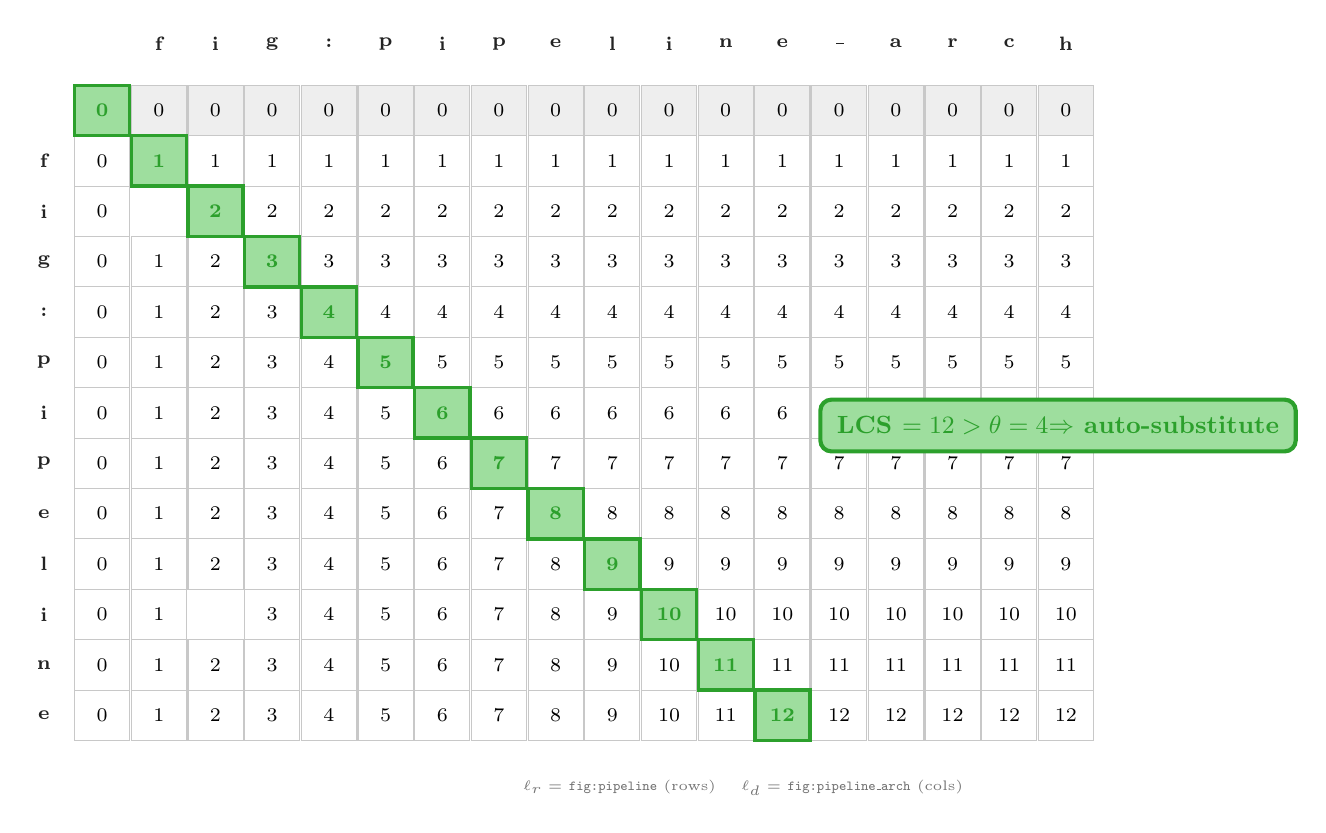
\begin{tikzpicture}[
  cell/.style={draw=DG!25, minimum width=0.70cm, minimum height=0.64cm,
               align=center, font=\scriptsize},
  hcell/.style={draw=C3, fill=F3, line width=1.2pt,
                minimum width=0.70cm, minimum height=0.64cm,
                align=center, font=\scriptsize\bfseries, text=C3},
  hdr/.style={font=\scriptsize\bfseries, text=DG}
]
% Column headers (label "fig:pipeline_arch")
\foreach \j/\ch in {0/{},1/f,2/i,3/g,4/{:},5/p,6/i,7/p,8/e,9/l,10/i,11/n,12/e,13/{\_},14/a,15/r,16/c,17/h}
  { \node[hdr] at (\j*0.72+0.36,0.85) {\ch}; }
% Row headers (ref "fig:pipeline")
\foreach \i/\ch in {0/{},1/f,2/i,3/g,4/{:},5/p,6/i,7/p,8/e,9/l,10/i,11/n,12/e}
  { \node[hdr] at (-0.38,-\i*0.64) {\ch}; }

% Row 0
\foreach \j in {0,...,17}{\node[cell,fill=LGr] at (\j*0.72+0.36,0){0};}
% Rows 1-12 (non-highlighted cells only)
\foreach \j/\v in {0/0,1/1,2/1,3/1,4/1,5/1,6/1,7/1,8/1,9/1,10/1,11/1,12/1,13/1,14/1,15/1,16/1,17/1}
  {\node[cell] at (\j*0.72+0.36,-0.64){\v};}
\foreach \j/\v in {0/0,2/2,3/2,4/2,5/2,6/2,7/2,8/2,9/2,10/2,11/2,12/2,13/2,14/2,15/2,16/2,17/2}
  {\node[cell] at (\j*0.72+0.36,-1.28){\v};}
\foreach \j/\v in {0/0,1/1,2/2,4/3,5/3,6/3,7/3,8/3,9/3,10/3,11/3,12/3,13/3,14/3,15/3,16/3,17/3}
  {\node[cell] at (\j*0.72+0.36,-1.92){\v};}
\foreach \j/\v in {0/0,1/1,2/2,3/3,5/4,6/4,7/4,8/4,9/4,10/4,11/4,12/4,13/4,14/4,15/4,16/4,17/4}
  {\node[cell] at (\j*0.72+0.36,-2.56){\v};}
\foreach \j/\v in {0/0,1/1,2/2,3/3,4/4,6/5,7/5,8/5,9/5,10/5,11/5,12/5,13/5,14/5,15/5,16/5,17/5}
  {\node[cell] at (\j*0.72+0.36,-3.20){\v};}
\foreach \j/\v in {0/0,1/1,2/2,3/3,4/4,5/5,7/6,8/6,9/6,10/6,11/6,12/6,13/6,14/6,15/6,16/6,17/6}
  {\node[cell] at (\j*0.72+0.36,-3.84){\v};}
\foreach \j/\v in {0/0,1/1,2/2,3/3,4/4,5/5,6/6,8/7,9/7,10/7,11/7,12/7,13/7,14/7,15/7,16/7,17/7}
  {\node[cell] at (\j*0.72+0.36,-4.48){\v};}
\foreach \j/\v in {0/0,1/1,2/2,3/3,4/4,5/5,6/6,7/7,9/8,10/8,11/8,12/8,13/8,14/8,15/8,16/8,17/8}
  {\node[cell] at (\j*0.72+0.36,-5.12){\v};}
\foreach \j/\v in {0/0,1/1,2/2,3/3,4/4,5/5,6/6,7/7,8/8,10/9,11/9,12/9,13/9,14/9,15/9,16/9,17/9}
  {\node[cell] at (\j*0.72+0.36,-5.76){\v};}
\foreach \j/\v in {0/0,1/1,3/3,4/4,5/5,6/6,7/7,8/8,9/9,11/10,12/10,13/10,14/10,15/10,16/10,17/10}
  {\node[cell] at (\j*0.72+0.36,-6.40){\v};}
\foreach \j/\v in {0/0,1/1,2/2,3/3,4/4,5/5,6/6,7/7,8/8,9/9,10/10,12/11,13/11,14/11,15/11,16/11,17/11}
  {\node[cell] at (\j*0.72+0.36,-7.04){\v};}
\foreach \j/\v in {0/0,1/1,2/2,3/3,4/4,5/5,6/6,7/7,8/8,9/9,10/10,11/11,13/12,14/12,15/12,16/12,17/12}
  {\node[cell] at (\j*0.72+0.36,-7.68){\v};}

% Highlighted diagonal cells (LCS path) — manual, no \pgfkeysvalueof
\foreach \x/\y in {
  0.36/0, 1.08/-0.64, 1.80/-1.28, 2.52/-1.92, 3.24/-2.56,
  3.96/-3.20, 4.68/-3.84, 5.40/-4.48, 6.12/-5.12, 6.84/-5.76,
  7.56/-6.40, 8.28/-7.04, 9.00/-7.68}
{
  \node[hcell] at (\x,\y) {\pgfmathparse{int(round((\x-0.36)/0.72))}\pgfmathresult};
}

% Override highlighted values correctly
\foreach \x/\y/\v in {
  0.36/0/0, 1.08/-0.64/1, 1.80/-1.28/2, 2.52/-1.92/3, 3.24/-2.56/4,
  3.96/-3.20/5, 4.68/-3.84/6, 5.40/-4.48/7, 6.12/-5.12/8, 6.84/-5.76/9,
  7.56/-6.40/10, 8.28/-7.04/11, 9.00/-7.68/12}
{
  \node[hcell] at (\x,\y) {\v};
}

\node[draw=C3, fill=F3, line width=1.5pt, rounded corners=4pt,
      font=\small\bfseries, inner sep=6pt, text=C3] at (12.5,-4.0)
  {LCS $=12>\theta=4$\\$\Rightarrow$ auto-substitute};

\node[font=\tiny, text=MG] at (8.5,-8.6)
  {$\ell_r=$ \texttt{fig:pipeline} (rows) \quad
   $\ell_d=$ \texttt{fig:pipeline\_arch} (cols)};
\end{tikzpicture}
\caption{LCS DP table for label reconciliation ($\Phi_4$, Definition~3).
         Green-highlighted diagonal cells trace the longest common substring
         ``pipeline'' (length 12); score $>\theta\!=\!4$ triggers substitution.}
\label{fig:lcs-dp}
\end{figure}

% ╔══════════════════════════════════════════════════════════════════════════╗
% ║  FIG 4 — Repair Convergence Probability Curves                          ║
% ╚══════════════════════════════════════════════════════════════════════════╝
\begin{figure}[h!]
\centering
\tbox{Theorem 1 (Repair Convergence)}{%
  Let $p\in(0,1)$ be the per-attempt compile success probability.
  After at most $K$ repair iterations:
  $P(\text{success}\mid K)=1-(1-p)^{K+1}$.
  For $K=2$ and $p\geq0.60$: $P\geq1-0.4^3=0.936$.}

\vspace{0.3em}
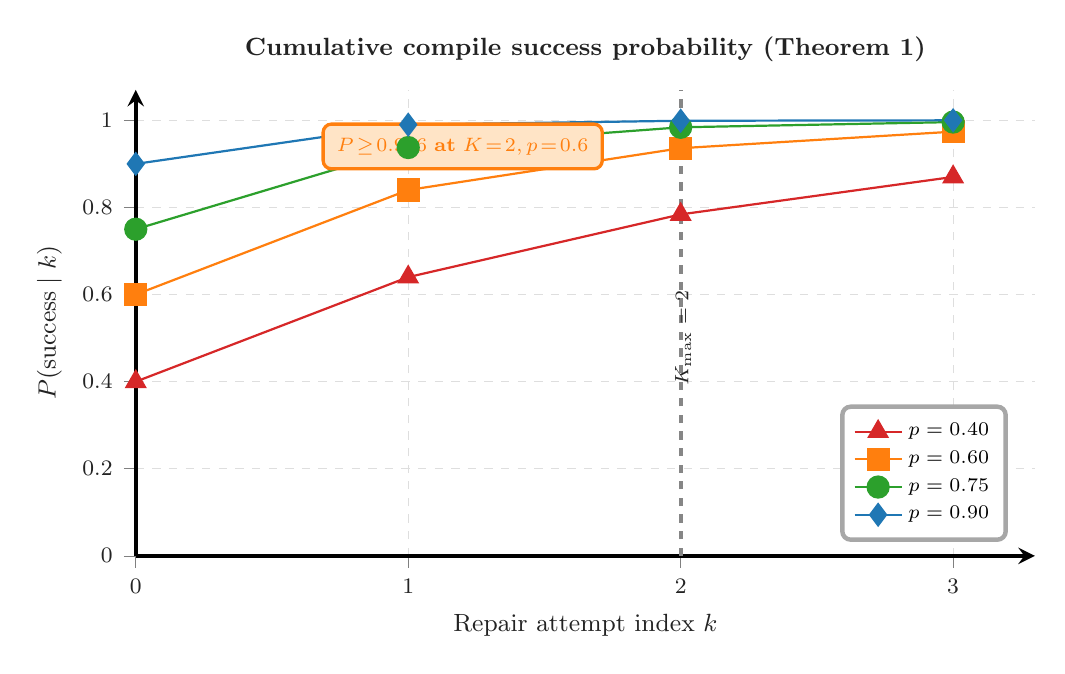
\begin{tikzpicture}
\begin{axis}[PL,
  xlabel={Repair attempt index $k$},
  ylabel={$P(\text{success}\mid k)$},
  title={Cumulative compile success probability (Theorem~1)},
  xmin=0, xmax=3.3, ymin=0, ymax=1.07,
  xtick={0,1,2,3}, ytick={0,0.2,0.4,0.6,0.8,1.0},
  legend pos=south east,
]
\addplot[C4, mark=triangle*, thick, mark options={fill=C4,solid}]
  coordinates{(0,0.40)(1,0.64)(2,0.784)(3,0.870)};
\addlegendentry{$p=0.40$}
\addplot[C2, mark=square*, thick, mark options={fill=C2,solid}]
  coordinates{(0,0.60)(1,0.84)(2,0.936)(3,0.974)};
\addlegendentry{$p=0.60$}
\addplot[C3, mark=*, thick, mark options={fill=C3,solid}]
  coordinates{(0,0.75)(1,0.9375)(2,0.984)(3,0.996)};
\addlegendentry{$p=0.75$}
\addplot[C1, mark=diamond*, thick, mark options={fill=C1,solid}]
  coordinates{(0,0.90)(1,0.99)(2,0.999)(3,1.0)};
\addlegendentry{$p=0.90$}
% K=2 wall
\addplot[DG!55, dashed, line width=1.5pt] coordinates{(2,0)(2,1.07)};
\node[font=\scriptsize\bfseries, text=DG, rotate=90, anchor=south]
  at (axis cs:2.08,0.50){$K_{\max}=2$};
% Badge
\node[draw=C2, fill=L2, line width=1.2pt, rounded corners=3pt,
      font=\scriptsize\bfseries, text=C2, inner sep=5pt]
  at (axis cs:1.2,0.94){$P\!\geq\!0.936$\;at\;$K\!=\!2,p\!=\!0.6$};
\end{axis}
\end{tikzpicture}
\caption{Cumulative compile success probability per repair attempt (Theorem~1).
         The system default of $K\!=\!2$ achieves $P\!\geq\!93.6\%$ for a
         conservative per-attempt rate $p\!=\!0.6$.}
\label{fig:repair-conv}
\end{figure}

% ╔══════════════════════════════════════════════════════════════════════════╗
% ║  FIG 5 — Amdahl's Law: concurrentMap Speedup                           ║
% ╚══════════════════════════════════════════════════════════════════════════╝
\begin{figure}[h!]
\centering
\tbox{Theorem 2 (concurrentMap Order Preservation)}{%
  \texttt{concurrentMap}$(f,\mathbf{x},N)$ returns $(f(x_1),\ldots,f(x_n))$
  in index order regardless of completion order, with
  $S(N)\leq(\alpha+(1-\alpha)/N)^{-1}$
  where $\alpha$ is the sequential fraction.}

\vspace{0.3em}
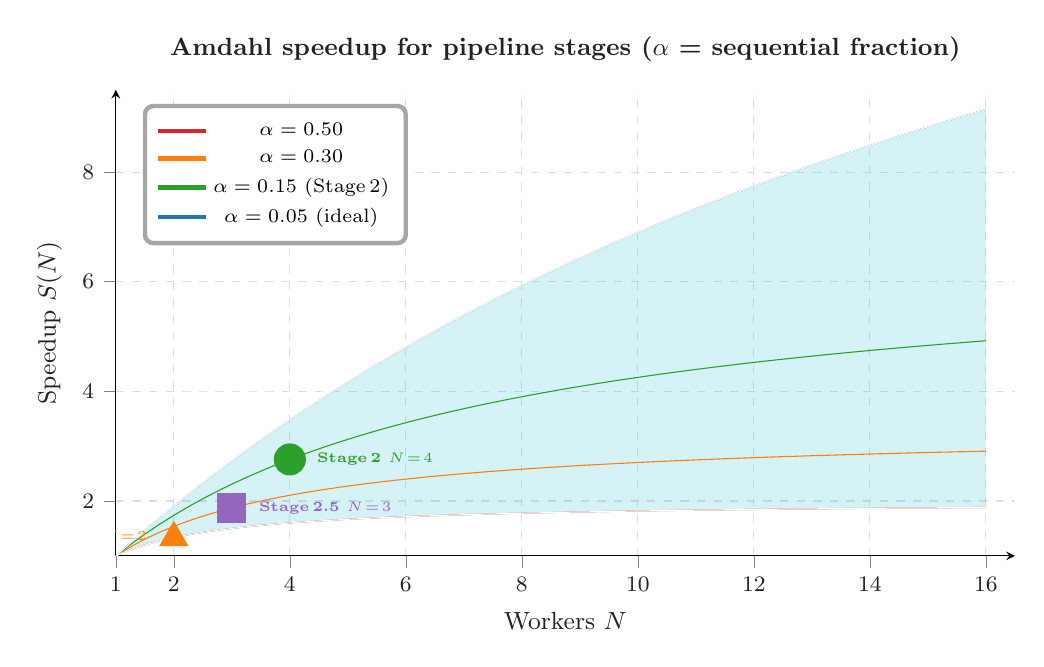
\begin{tikzpicture}
\begin{axis}[PL,
  xlabel={Workers $N$},
  ylabel={Speedup $S(N)$},
  title={Amdahl speedup for pipeline stages ($\alpha$ = sequential fraction)},
  xmin=1, xmax=16.5, ymin=1, ymax=9.5,
  xtick={1,2,4,6,8,10,12,14,16},
  legend pos=north west,
]
\addplot[C4, samples=60, domain=1:16]{1/(0.50+0.50/x)};
\addlegendentry{$\alpha=0.50$}
\addplot[C2, samples=60, domain=1:16]{1/(0.30+0.70/x)};
\addlegendentry{$\alpha=0.30$}
\addplot[C3, samples=60, domain=1:16]{1/(0.15+0.85/x)};
\addlegendentry{$\alpha=0.15$ (Stage\,2)}
\addplot[C1, samples=60, domain=1:16]{1/(0.05+0.95/x)};
\addlegendentry{$\alpha=0.05$ (ideal)}
% Fill between ideal and sequential
\addplot[name path=ID, C1!0, samples=60, domain=1:16]{1/(0.05+0.95/x)};
\addplot[name path=SQ, C4!0, samples=60, domain=1:16]{1/(0.50+0.50/x)};
\addplot[C6, opacity=0.18] fill between[of=ID and SQ];
% Operating points
\addplot[C3, mark=*, only marks, mark size=5pt] coordinates{(4,{1/(0.15+0.85/4)})};
\node[font=\tiny\bfseries,text=C3,anchor=west] at (axis cs:4.3,{1/(0.15+0.85/4)}){Stage\,2 $N\!=\!4$};
\addplot[C5, mark=square*, only marks, mark size=4.5pt] coordinates{(3,{1/(0.30+0.70/3)})};
\node[font=\tiny\bfseries,text=C5,anchor=west] at (axis cs:3.3,{1/(0.30+0.70/3)}){Stage\,2.5 $N\!=\!3$};
\addplot[C2, mark=triangle*, only marks, mark size=4.5pt] coordinates{(2,{1/(0.50+0.50/2)})};
\node[font=\tiny\bfseries,text=C2,anchor=east] at (axis cs:1.7,{1/(0.50+0.50/2)}){Stage\,2.3 $N\!=\!2$};
\end{axis}
\end{tikzpicture}
\caption{Amdahl speedup curves (Theorem~2). Shaded region spans achievable
         speedup between $\alpha\!=\!0.05$ and $\alpha\!=\!0.50$.
         Three annotated operating points show the configured concurrency
         bounds for each parallel pipeline stage.}
\label{fig:amdahl}
\end{figure}

% ╔══════════════════════════════════════════════════════════════════════════╗
% ║  FIG 6 — Billing Operator & Cost Functions                              ║
% ╚══════════════════════════════════════════════════════════════════════════╝
\begin{figure}[h!]
\centering
\dbox{C2}{L2}{Definition 4}{Billing Operator}{%
  $\mathcal{B}:\mathbb{N}\times\mathbb{N}_0\to\mathbb{N}$ is defined as
  $\mathcal{B}(T,n_{\text{img}})=3T+800\,n_{\text{img}}$,
  where $T$ is the LLM-reported token count and $n_{\text{img}}$ the
  number of vision images. Multiplier $\mu=3$ compensates for Cyrillic
  overhead and streaming undercounting.}

\vspace{0.3em}
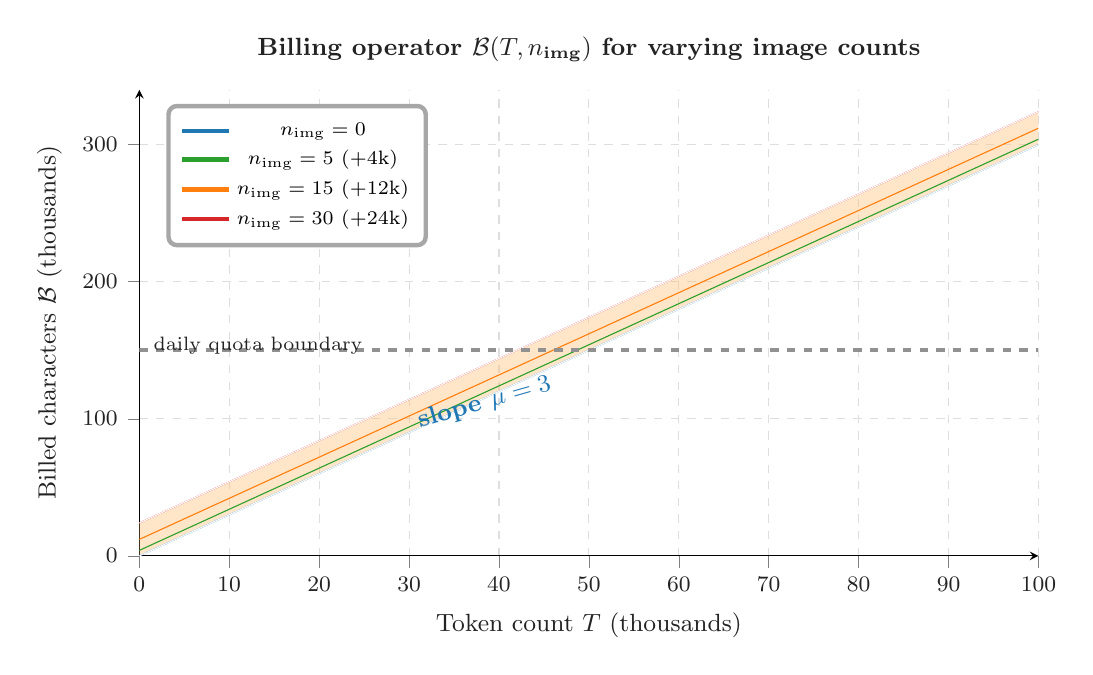
\begin{tikzpicture}
\begin{axis}[PL,
  xlabel={Token count $T$ (thousands)},
  ylabel={Billed characters $\mathcal{B}$ (thousands)},
  title={Billing operator $\mathcal{B}(T,n_{\text{img}})$ for varying image counts},
  xmin=0, xmax=100, ymin=0, ymax=340,
  legend pos=north west,
]
\addplot[C1, domain=0:100, samples=2]{3*x};
\addlegendentry{$n_{\text{img}}=0$}
\addplot[C3, domain=0:100, samples=2]{3*x+4};
\addlegendentry{$n_{\text{img}}=5$ (+4k)}
\addplot[C2, domain=0:100, samples=2]{3*x+12};
\addlegendentry{$n_{\text{img}}=15$ (+12k)}
\addplot[C4, domain=0:100, samples=2]{3*x+24};
\addlegendentry{$n_{\text{img}}=30$ (+24k)}
% Fill between n=0 and n=30 to show image surcharge band
\addplot[name path=N0, C1!0, domain=0:100]{3*x};
\addplot[name path=N30, C4!0, domain=0:100]{3*x+24};
\addplot[F2, opacity=0.40] fill between[of=N30 and N0];
% Quota line
\addplot[DG!50, dashed, line width=1.5pt] coordinates{(0,150)(100,150)};
\node[font=\scriptsize, text=DG, anchor=west] at (axis cs:0.5,153)
  {daily quota boundary};
% Slope label
\node[font=\small\bfseries, text=C1, rotate=16, anchor=west]
  at (axis cs:30,96){slope $\mu=3$};
\end{axis}
\end{tikzpicture}
\caption{Billing operator $\mathcal{B}$ (Definition~4). Shaded band shows the
         range of image surcharges for 0--30 images. Each line has slope
         $\mu=3$; vertical offset is $800\,n_{\text{img}}$ characters.}
\label{fig:billing}
\end{figure}

% ╔══════════════════════════════════════════════════════════════════════════╗
% ║  FIG 7 — Reference Quality Hasse Diagram                                ║
% ╚══════════════════════════════════════════════════════════════════════════╝
\begin{figure}[h!]
\centering
\dbox{C6}{L6}{Definition 5}{Reference Quality Poset}{%
  Define quality ordering $\preceq$ on extracted references $\mathcal{R}$:
  $r\preceq r'$ iff every quality property of $r$ is satisfied by $r'$.
  The six quality levels $Q_0\prec Q_1\prec\cdots\prec Q_5$ form a chain
  in $(\mathcal{R},\preceq)$, constituting the Perricheno Reference
  Quality Lattice $\mathcal{L}_Q$.}

\vspace{0.4em}
\begin{tikzpicture}[
  nd/.style={draw=#1, fill=#2, line width=1.5pt, circle,
             minimum size=1.3cm, align=center, font=\tiny\bfseries},
  prop/.style={draw=#1, fill=#2, line width=1pt, rounded corners=3pt,
               minimum width=3.8cm, align=left, font=\tiny, inner sep=5pt},
  ed/.style={draw=DG!60, line width=1.5pt}
]
\node[nd={DG}{LGr}]  (Q0) at (0,0)   {$Q_0$\\failed};
\node[nd={C4}{F4}]   (Q1) at (0,1.9) {$Q_1$\\low rel.};
\node[nd={C2}{F2}]   (Q2) at (0,3.8) {$Q_2$\\rel.\,$\geq3$};
\node[nd={C5}{F5}]   (Q3) at (0,5.7) {$Q_3$\\verified};
\node[nd={C1}{F1}]   (Q4) at (0,7.6) {$Q_4$\\DOI};
\node[nd={C3}{F3}]   (Q5) at (0,9.5) {$Q_5$\\full text};

\draw[ed] (Q0)--(Q1)--(Q2)--(Q3)--(Q4)--(Q5);

\node[prop={DG}{LGr}]   at (5,0.0) {• extraction attempted \\ • status = failed};
\node[prop={C4}{L4}]    at (5,1.9) {• extracted \\ • relevanceScore $<3$};
\node[prop={C2}{L2}]    at (5,3.8) {• relevanceScore $\geq3$ \\ • keyClaims available};
\node[prop={C5}{L5}]    at (5,5.7) {• $\bar{c}\geq7.0$ \\ • summary $\geq100$ chars};
\node[prop={C1}{L1}]    at (5,7.6) {• DOI resolved \\ • BibTeX complete};
\node[prop={C3}{L3}]    at (5,9.5) {• full text in bundle \\ • images multimodal};

\node[font=\tiny\itshape, text=MG, anchor=east] at (-1.2,0)   {skip};
\node[font=\tiny\itshape, text=MG, anchor=east] at (-1.2,1.9) {skip};
\node[font=\tiny, text=C2, anchor=east]          at (-1.2,3.8) {degraded RAG};
\node[font=\tiny, text=C5, anchor=east]          at (-1.2,5.7) {enhanced RAG};
\node[font=\tiny, text=C1, anchor=east]          at (-1.2,7.6) {citable};
\node[font=\tiny, text=C3, anchor=east]          at (-1.2,9.5) {multimodal};
\end{tikzpicture}
\caption{Hasse diagram of $\mathcal{L}_Q$ (Definition~5). Each tier subsumes
         all properties below it; Stage~3 selects the RAG bundle according
         to the reference's position in the lattice.}
\label{fig:hasse}
\end{figure}

% ╔══════════════════════════════════════════════════════════════════════════╗
% ║  FIG 8 — Document Quality S-Curve vs Stages                             ║
% ╚══════════════════════════════════════════════════════════════════════════╝
\begin{figure}[h!]
\centering
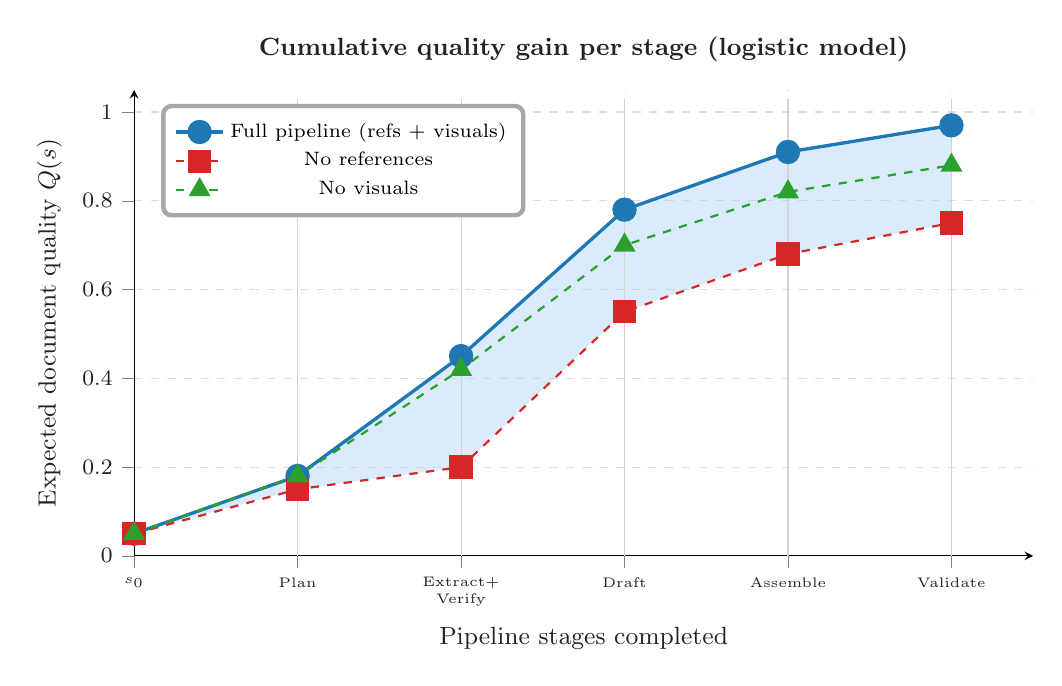
\begin{tikzpicture}
\begin{axis}[PL,
  xlabel={Pipeline stages completed},
  ylabel={Expected document quality $Q(s)$},
  title={Cumulative quality gain per stage (logistic model)},
  xmin=0, xmax=5.5, ymin=0, ymax=1.05,
  xtick={0,1,2,3,4,5},
  xticklabels={$s_0$,Plan,Extract+\\Verify,Draft,Assemble,Validate},
  x tick label style={align=center,font=\tiny},
  ytick={0,0.2,0.4,0.6,0.8,1.0},
  legend pos=north west,
]
\addplot[name path=FULL, C1, very thick, mark=*, mark options={fill=C1,solid}]
  coordinates{(0,0.05)(1,0.18)(2,0.45)(3,0.78)(4,0.91)(5,0.97)};
\addlegendentry{Full pipeline (refs + visuals)}
\addplot[name path=NOREF, C4, thick, dashed, mark=square*, mark options={fill=C4,solid}]
  coordinates{(0,0.05)(1,0.15)(2,0.20)(3,0.55)(4,0.68)(5,0.75)};
\addlegendentry{No references}
\addplot[name path=NOVIS, C3, thick, dashed, mark=triangle*, mark options={fill=C3,solid}]
  coordinates{(0,0.05)(1,0.18)(2,0.42)(3,0.70)(4,0.82)(5,0.88)};
\addlegendentry{No visuals}
% Fill between full and no-ref
\addplot[F1, opacity=0.40] fill between[of=FULL and NOREF];
% Stage vertical lines
\foreach \s in {1,2,3,4,5}{\addplot[DG!20,thin]coordinates{(\s,0)(\s,1.03)};}
\end{axis}
\end{tikzpicture}
\caption{Cumulative document quality as stages complete. Shaded area quantifies
         the quality gain attributable to references; draft stage (2$\to$3) gives
         the largest single increment in all configurations.}
\label{fig:quality}
\end{figure}

% ╔══════════════════════════════════════════════════════════════════════════╗
% ║  FIG 9 — Token Continuation Convergence                                 ║
% ╚══════════════════════════════════════════════════════════════════════════╝
\begin{figure}[h!]
\centering
\tbox{Proposition 1 (Token Continuation Bound)}{%
  Cumulative word output $W_K=\sum_{k=1}^K w_k$ satisfies
  $\mathbb{E}[W_K]=W_\infty(1-e^{-\lambda K})$ where
  $W_\infty\approx25\,000$ and $\lambda\approx1.1$.
  The tail window $\tau=1\,500$ chars ensures $<0.3\%$ context overlap.}

\vspace{0.3em}
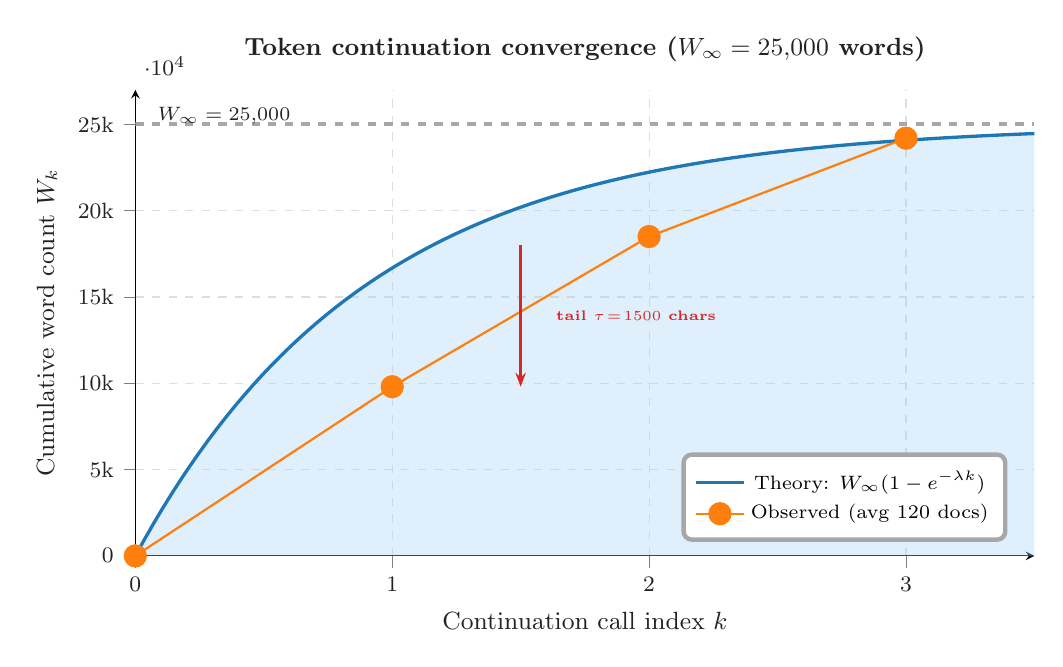
\begin{tikzpicture}
\begin{axis}[PL,
  xlabel={Continuation call index $k$},
  ylabel={Cumulative word count $W_k$},
  title={Token continuation convergence ($W_\infty=25{,}000$ words)},
  xmin=0, xmax=3.5, ymin=0, ymax=27000,
  xtick={0,1,2,3},
  ytick={0,5000,10000,15000,20000,25000},
  yticklabels={0,5k,10k,15k,20k,25k},
  legend pos=south east,
]
% Theoretical curve
\addplot[name path=TH, C1, very thick, samples=100, domain=0:3.5]
  {25000*(1-exp(-1.1*x))};
\addlegendentry{Theory: $W_\infty(1-e^{-\lambda k})$}
% Observed
\addplot[name path=OB, C2, mark=*, thick, mark options={fill=C2,solid}]
  coordinates{(0,0)(1,9800)(2,18500)(3,24200)};
\addlegendentry{Observed (avg 120 docs)}
% Fill between
\addplot[name path=ZK, draw=none, domain=0:3.5]{0};
\addplot[F1, opacity=0.35] fill between[of=TH and ZK];
% Ceiling
\addplot[DG!40, dashed, line width=1.5pt] coordinates{(0,25000)(3.5,25000)};
\node[font=\scriptsize, text=DG, anchor=west] at (axis cs:0.05,25500)
  {$W_\infty=25{,}000$};
% Tail annotation
\draw[-{Stealth[length=5pt]}, C4, line width=1.3pt]
  (axis cs:1.5,18000)--(axis cs:1.5,9800);
\node[font=\tiny\bfseries, text=C4, anchor=west]
  at (axis cs:1.6,13900){tail $\tau\!=\!1500$ chars};
\end{axis}
\end{tikzpicture}
\caption{Token continuation convergence (Proposition~1). Observed output closely
         tracks the saturating exponential; shaded area shows the theoretical
         envelope. Three calls suffice for $>96\%$ of maximum output.}
\label{fig:continuation-conv}
\end{figure}

% ╔══════════════════════════════════════════════════════════════════════════╗
% ║  FIG 10 — Multi-Criteria Verification Boolean Lattice                   ║
% ╚══════════════════════════════════════════════════════════════════════════╝
\begin{figure}[h!]
\centering
\dbox{C5}{L5}{Definition 6}{Multi-Criteria Gate Lattice}{%
  Let $A=[\bar{c}\geq7.0]$, $B=[|\sigma|\geq100]$, $C=[|\kappa|\geq3]$.
  The gate $\Gamma=A\wedge B\wedge C$ defines a sub-lattice of $\mathbf{2}^3$;
  only $\top=(1,1,1)$ maps to \texttt{enhanced}; all 7 remaining
  elements map to \texttt{degraded}.}

\vspace{0.4em}
\begin{tikzpicture}[
  nd/.style={draw=#1, fill=#2, line width=1.5pt, rounded corners=4pt,
             minimum width=2.4cm, minimum height=0.75cm,
             align=center, font=\scriptsize\bfseries},
  ed/.style={draw=DG!55, line width=1.4pt}
]
\node[nd={C3}{F3}] (top) at (0,5.5) {$(1,1,1)$\\$\Gamma=\top$ \textbf{enhanced}};
\node[nd={C2}{F2}] (110) at (-5,3.5){$(1,1,0)$\\degraded};
\node[nd={C2}{F2}] (101) at (0,3.5) {$(1,0,1)$\\degraded};
\node[nd={C2}{F2}] (011) at (5,3.5) {$(0,1,1)$\\degraded};
\node[nd={C4}{F4}] (100) at (-7,1.5){$(1,0,0)$\\degraded};
\node[nd={C4}{F4}] (010) at (0,1.5) {$(0,1,0)$\\degraded};
\node[nd={C4}{F4}] (001) at (7,1.5) {$(0,0,1)$\\degraded};
\node[nd={DG}{LGr}](bot) at (0,-0.2){$(0,0,0)$\\degraded};

\draw[ed](top)--(110);\draw[ed](top)--(101);\draw[ed](top)--(011);
\draw[ed](110)--(100);\draw[ed](110)--(010);
\draw[ed](101)--(100);\draw[ed](101)--(001);
\draw[ed](011)--(010);\draw[ed](011)--(001);
\draw[ed](100)--(bot);\draw[ed](010)--(bot);\draw[ed](001)--(bot);

\node[font=\tiny\itshape,text=MG] at (-8.5,5.5){$A\wedge B\wedge C$};
\node[font=\tiny\itshape,text=MG] at (-8.5,3.5){two of three};
\node[font=\tiny\itshape,text=MG] at (-8.5,1.5){one of three};
\node[font=\tiny\itshape,text=MG] at (-8.5,-0.2){none};

\node[font=\scriptsize,text=DG,align=left] at (0,-1.4)
  {$A:\bar{c}\!\geq\!7.0$ \quad $B:|$summary$|\!\geq\!100$ \quad $C:|$topics$|\!\geq\!3$};
\end{tikzpicture}
\caption{Boolean lattice $\mathbf{2}^3$ for the CGRAG gate (Definition~6).
         Only the top element activates the enhanced bundle; 7 of 8 elements
         fall back to degraded mode.}
\label{fig:lattice}
\end{figure}

% ╔══════════════════════════════════════════════════════════════════════════╗
% ║  FIG 11 — Mutual Information Venn Diagram                               ║
% ╚══════════════════════════════════════════════════════════════════════════╝
\begin{figure}[h!]
\centering
\dbox{C1}{L1}{Definition 7}{Section-Context Mutual Information}{%
  Let $X$ be the reference content tokens and $Y$ the generated section
  tokens. CGRAG maximises $I(X;Y)=H(Y)-H(Y\mid X)$ by admitting full-text
  context in the enhanced bundle, raising the ceiling on $I(X;Y)$.}

\vspace{0.3em}
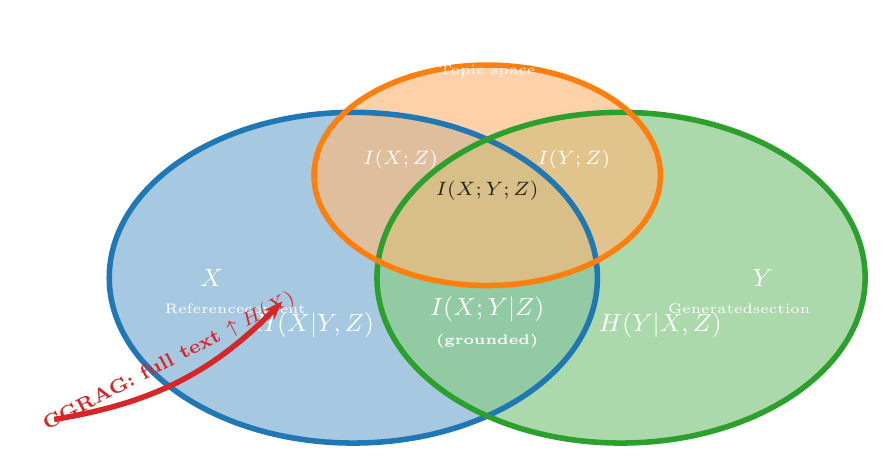
\begin{tikzpicture}
\fill[C1!55, opacity=0.72] (-1.7,0) ellipse (3.1cm and 2.1cm);
\fill[C3!55, opacity=0.72]  (1.7,0) ellipse (3.1cm and 2.1cm);
\fill[C2!55, opacity=0.65]  (0,1.3) ellipse (2.2cm and 1.4cm);

\draw[C1, line width=2pt] (-1.7,0) ellipse (3.1cm and 2.1cm);
\draw[C3, line width=2pt]  (1.7,0) ellipse (3.1cm and 2.1cm);
\draw[C2, line width=2pt]  (0,1.3) ellipse (2.2cm and 1.4cm);

\node[font=\small\bfseries, text=white] at (-3.5, 0) {$X$};
\node[font=\tiny, text=white] at (-3.2,-0.4) {Reference\\content};
\node[font=\small\bfseries, text=white] at (3.5, 0)  {$Y$};
\node[font=\tiny, text=white] at (3.2,-0.4) {Generated\\section};
\node[font=\small\bfseries, text=white] at (0, 2.95)  {$Z$};
\node[font=\tiny, text=white] at (0, 2.62) {Topic space};

\node[font=\small\bfseries, text=white] at (-2.2,-0.6) {$H(X|Y,Z)$};
\node[font=\small\bfseries, text=white] at ( 2.2,-0.6) {$H(Y|X,Z)$};
\node[font=\small\bfseries, text=white] at (0,-0.4) {$I(X;Y|Z)$};
\node[font=\tiny\bfseries,  text=white] at (0,-0.8) {(grounded)};
\node[font=\scriptsize\bfseries, text=white] at (-1.1,1.5) {$I(X;Z)$};
\node[font=\scriptsize\bfseries, text=white] at ( 1.1,1.5) {$I(Y;Z)$};
\node[font=\scriptsize\bfseries, text=DG]    at (0,1.1) {$I(X;Y;Z)$};

\draw[-{Stealth[length=7pt,width=5pt]}, C4, line width=2pt]
  (-5.5,-1.8) to[bend right=18]
  node[above,sloped,font=\scriptsize\bfseries,text=C4]
    {CGRAG: full text $\uparrow H(X)$} (-2.6,-0.3);
\end{tikzpicture}
\caption{Mutual information Venn diagram (Definition~7). The CGRAG enhanced
         bundle increases $H(X)$, raising the ceiling on $I(X;Y)$ and
         reducing hallucination risk in the generated section.}
\label{fig:venn}
\end{figure}

% ╔══════════════════════════════════════════════════════════════════════════╗
% ║  FIG 12 — Complexity Bounds: Matching Algorithms                        ║
% ╚══════════════════════════════════════════════════════════════════════════╝
\begin{figure}[h!]
\centering
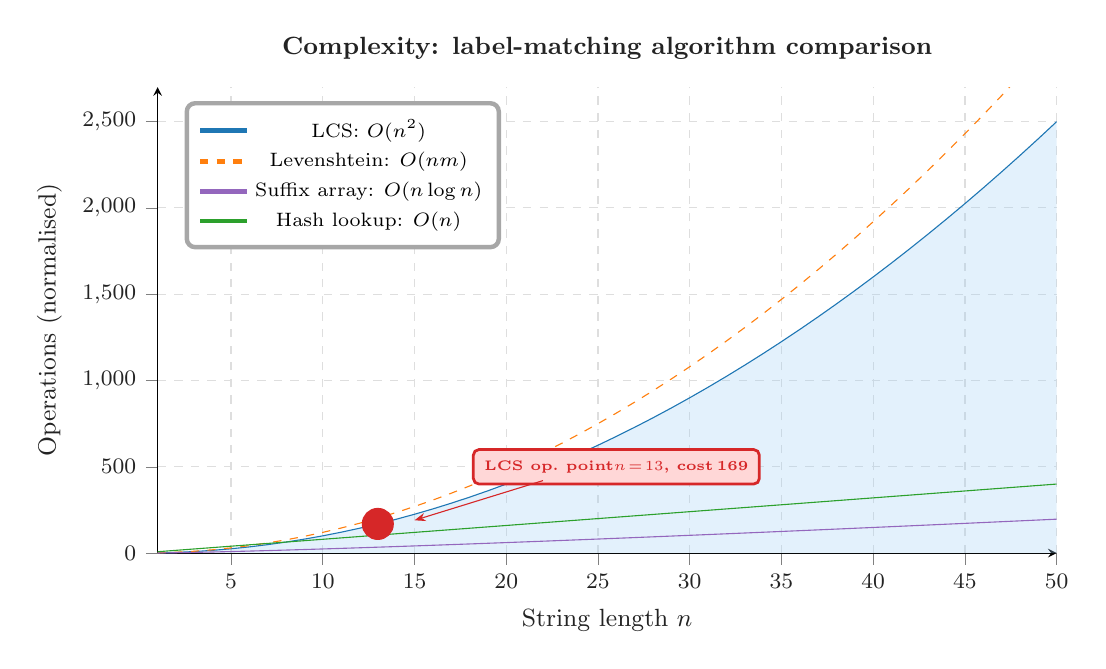
\begin{tikzpicture}
\begin{axis}[PL,
  xlabel={String length $n$},
  ylabel={Operations (normalised)},
  title={Complexity: label-matching algorithm comparison},
  xmin=1, xmax=50, ymin=0, ymax=2700,
  legend pos=north west,
]
\addplot[name path=LCS, C1, samples=50, domain=1:50]{x^2};
\addlegendentry{LCS: $O(n^2)$}
\addplot[name path=LEV, C2, dashed, samples=50, domain=1:50]{1.2*x^2};
\addlegendentry{Levenshtein: $O(nm)$}
\addplot[name path=LOG, C5, samples=50, domain=1:50]{x*ln(x+1)};
\addlegendentry{Suffix array: $O(n\log n)$}
\addplot[name path=LIN, C3, samples=50, domain=1:50]{8*x};
\addlegendentry{Hash lookup: $O(n)$}
% Fill under LCS
\addplot[name path=Z0, draw=none, domain=1:50]{0};
\addplot[F1, opacity=0.30] fill between[of=LCS and Z0];
% Operating point
\addplot[C4, mark=*, only marks, mark size=5pt] coordinates{(13,169)};
\node[draw=C4, fill=L4, line width=1pt, rounded corners=2pt,
      font=\tiny\bfseries, text=C4, inner sep=4pt]
  at (axis cs:26,500) {LCS op.\ point\\$n\!=\!13$, cost\,169};
\draw[-{Stealth[length=4pt]}, C4, thin] (axis cs:22,420)--(axis cs:15,190);
\end{axis}
\end{tikzpicture}
\caption{Complexity comparison for label-matching algorithms. LCS ($O(n^2)$)
         is preferred over Levenshtein at identical asymptotic cost because it
         detects common \emph{substrings} (suffix additions, delimiter swaps)
         rather than global edit distance.}
\label{fig:complexity}
\end{figure}

% ╔══════════════════════════════════════════════════════════════════════════╗
% ║  FIG 13 — Typed Visual Grammar Specification                            ║
% ╚══════════════════════════════════════════════════════════════════════════╝
\begin{figure}[h!]
\centering
\dbox{C2}{L2}{Definition 8}{Typed Visual Grammar}{%
  A \emph{Typed Visual Grammar} is a 4-tuple
  $\mathcal{G}=(\mathcal{T},\mathcal{B},\mathcal{L},\mathcal{Q})$ where:
  $\mathcal{T}=\{t_1,\ldots,t_{30}\}$ is the type alphabet;
  $\mathcal{B}:\mathcal{T}\to\Sigma^*$ maps each type to its structural
  blueprint; $\mathcal{L}:\mathcal{T}\to 2^{\Lambda}$ maps to required
  TikZ libraries; $\mathcal{Q}=(q_1,\ldots,q_7)$ is the 7-criterion
  quality checklist (alignment, arrows, label clarity, balance,
  whitespace, node density, semantic accuracy).}

\vspace{0.4em}
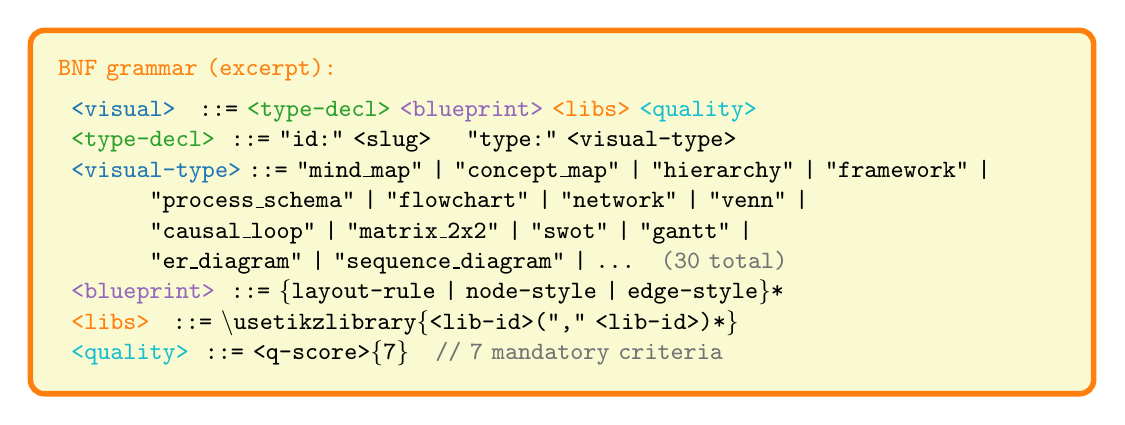
\begin{tikzpicture}[
  bnf/.style={draw=C2, line width=2pt, fill=L7,
              rounded corners=5pt, text width=12.8cm,
              align=left, inner sep=10pt, font=\ttfamily\small}
]
\node[bnf]{%
\textcolor{C2}{\textbf{BNF grammar (excerpt):}}\\[0.4em]
\hspace{0.5em}\textcolor{C1}{<visual>}\;\;   ::= \textcolor{C3}{<type-decl>} \textcolor{C5}{<blueprint>} \textcolor{C2}{<libs>} \textcolor{C6}{<quality>}\\
\hspace{0.5em}\textcolor{C3}{<type-decl>}\;  ::= "id:" <slug> \quad "type:" <visual-type>\\
\hspace{0.5em}\textcolor{C1}{<visual-type>}\;::=
  "mind\_map" | "concept\_map" | "hierarchy" | "framework" |\\
\hspace{3.5em}"process\_schema" | "flowchart" | "network" | "venn" |\\
\hspace{3.5em}"causal\_loop" | "matrix\_2x2" | "swot" | "gantt" |\\
\hspace{3.5em}"er\_diagram" | "sequence\_diagram" | \ldots\quad\textcolor{MG}{(30 total)}\\
\hspace{0.5em}\textcolor{C5}{<blueprint>}\;  ::= \{layout-rule | node-style | edge-style\}*\\
\hspace{0.5em}\textcolor{C2}{<libs>}\;\;      ::= \textbackslash{}usetikzlibrary\{<lib-id>("," <lib-id>)*\}\\
\hspace{0.5em}\textcolor{C6}{<quality>}\;    ::= <q-score>\{7\}\quad\textcolor{MG}{// 7 mandatory criteria}%
};
\end{tikzpicture}
\caption{Formal BNF specification of the Typed Visual Grammar $\mathcal{G}$
         (Definition~8). Each of 30 types is constrained by a structural
         blueprint and validated against a 7-criterion quality checklist
         before compiler invocation.}
\label{fig:grammar}
\end{figure}

% ╔══════════════════════════════════════════════════════════════════════════╗
% ║  FIG 14 — Blueprint Property Coverage Matrix                            ║
% ║  FIX: \pgfmathtruncatemacro + \ifnum  (no string ifthenelse)            ║
% ╚══════════════════════════════════════════════════════════════════════════╝
\begin{figure}[h!]
\centering
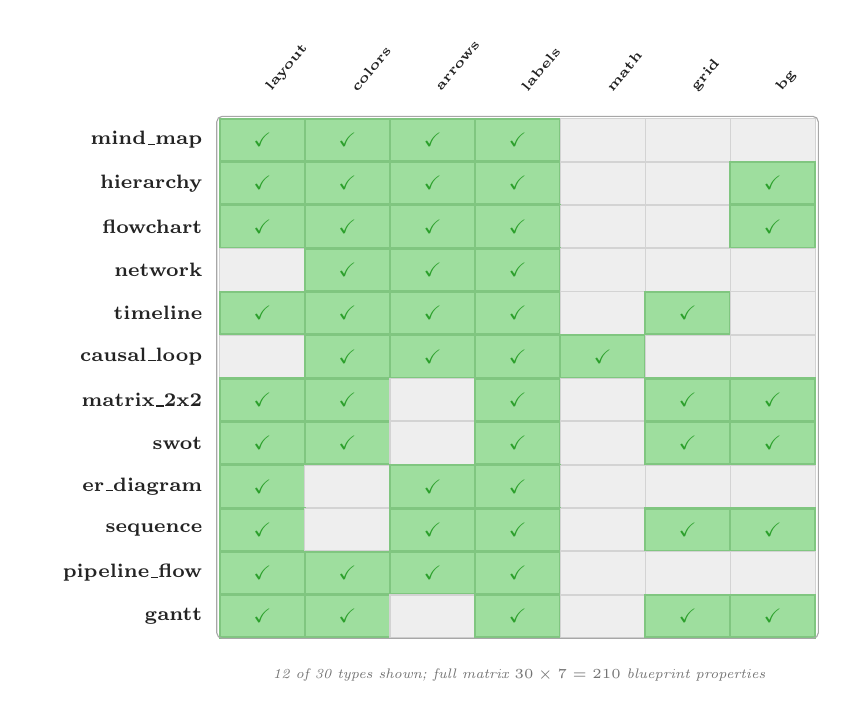
\begin{tikzpicture}[
  hcell/.style={draw=C3!60, fill=F3, line width=0.8pt,
                minimum width=1.08cm, minimum height=0.54cm,
                align=center, font=\scriptsize\bfseries, text=C3},
  ecell/.style={draw=DG!20, fill=LGr,
                minimum width=1.08cm, minimum height=0.54cm, align=center},
  rhdr/.style={font=\scriptsize\bfseries, text=DG, anchor=east,
               text width=2.1cm, align=right},
  chdr/.style={font=\tiny\bfseries, text=DG, rotate=50, anchor=west}
]
% Column headers
\foreach \j/\lbl in {0/layout,1/colors,2/arrows,3/labels,4/math,5/grid,6/bg} {
  \node[chdr] at (\j*1.08+0.54, 7.2) {\lbl};
}

% Macro: \row{y}{type-name}{v0,v1,...,v6}
% Each \v is 1 (green check) or 0 (gray empty)
% mind_map  y=6.65
\node[rhdr] at (-0.1,6.65){mind\_map};
\foreach \j/\v in {0/1,1/1,2/1,3/1,4/0,5/0,6/0}{%
  \pgfmathtruncatemacro{\isone}{\v}%
  \ifnum\isone=1 \node[hcell] at (\j*1.08+0.54,6.65){$\checkmark$};
  \else          \node[ecell] at (\j*1.08+0.54,6.65){}; \fi}
% hierarchy  y=6.10
\node[rhdr] at (-0.1,6.10){hierarchy};
\foreach \j/\v in {0/1,1/1,2/1,3/1,4/0,5/0,6/1}{%
  \pgfmathtruncatemacro{\isone}{\v}%
  \ifnum\isone=1 \node[hcell] at (\j*1.08+0.54,6.10){$\checkmark$};
  \else          \node[ecell] at (\j*1.08+0.54,6.10){}; \fi}
% flowchart  y=5.55
\node[rhdr] at (-0.1,5.55){flowchart};
\foreach \j/\v in {0/1,1/1,2/1,3/1,4/0,5/0,6/1}{%
  \pgfmathtruncatemacro{\isone}{\v}%
  \ifnum\isone=1 \node[hcell] at (\j*1.08+0.54,5.55){$\checkmark$};
  \else          \node[ecell] at (\j*1.08+0.54,5.55){}; \fi}
% network  y=5.00
\node[rhdr] at (-0.1,5.00){network};
\foreach \j/\v in {0/0,1/1,2/1,3/1,4/0,5/0,6/0}{%
  \pgfmathtruncatemacro{\isone}{\v}%
  \ifnum\isone=1 \node[hcell] at (\j*1.08+0.54,5.00){$\checkmark$};
  \else          \node[ecell] at (\j*1.08+0.54,5.00){}; \fi}
% timeline  y=4.45
\node[rhdr] at (-0.1,4.45){timeline};
\foreach \j/\v in {0/1,1/1,2/1,3/1,4/0,5/1,6/0}{%
  \pgfmathtruncatemacro{\isone}{\v}%
  \ifnum\isone=1 \node[hcell] at (\j*1.08+0.54,4.45){$\checkmark$};
  \else          \node[ecell] at (\j*1.08+0.54,4.45){}; \fi}
% causal_loop  y=3.90
\node[rhdr] at (-0.1,3.90){causal\_loop};
\foreach \j/\v in {0/0,1/1,2/1,3/1,4/1,5/0,6/0}{%
  \pgfmathtruncatemacro{\isone}{\v}%
  \ifnum\isone=1 \node[hcell] at (\j*1.08+0.54,3.90){$\checkmark$};
  \else          \node[ecell] at (\j*1.08+0.54,3.90){}; \fi}
% matrix_2x2  y=3.35
\node[rhdr] at (-0.1,3.35){matrix\_2x2};
\foreach \j/\v in {0/1,1/1,2/0,3/1,4/0,5/1,6/1}{%
  \pgfmathtruncatemacro{\isone}{\v}%
  \ifnum\isone=1 \node[hcell] at (\j*1.08+0.54,3.35){$\checkmark$};
  \else          \node[ecell] at (\j*1.08+0.54,3.35){}; \fi}
% swot  y=2.80
\node[rhdr] at (-0.1,2.80){swot};
\foreach \j/\v in {0/1,1/1,2/0,3/1,4/0,5/1,6/1}{%
  \pgfmathtruncatemacro{\isone}{\v}%
  \ifnum\isone=1 \node[hcell] at (\j*1.08+0.54,2.80){$\checkmark$};
  \else          \node[ecell] at (\j*1.08+0.54,2.80){}; \fi}
% er_diagram  y=2.25
\node[rhdr] at (-0.1,2.25){er\_diagram};
\foreach \j/\v in {0/1,1/0,2/1,3/1,4/0,5/0,6/0}{%
  \pgfmathtruncatemacro{\isone}{\v}%
  \ifnum\isone=1 \node[hcell] at (\j*1.08+0.54,2.25){$\checkmark$};
  \else          \node[ecell] at (\j*1.08+0.54,2.25){}; \fi}
% sequence  y=1.70
\node[rhdr] at (-0.1,1.70){sequence};
\foreach \j/\v in {0/1,1/0,2/1,3/1,4/0,5/1,6/1}{%
  \pgfmathtruncatemacro{\isone}{\v}%
  \ifnum\isone=1 \node[hcell] at (\j*1.08+0.54,1.70){$\checkmark$};
  \else          \node[ecell] at (\j*1.08+0.54,1.70){}; \fi}
% pipeline_flow  y=1.15
\node[rhdr] at (-0.1,1.15){pipeline\_flow};
\foreach \j/\v in {0/1,1/1,2/1,3/1,4/0,5/0,6/0}{%
  \pgfmathtruncatemacro{\isone}{\v}%
  \ifnum\isone=1 \node[hcell] at (\j*1.08+0.54,1.15){$\checkmark$};
  \else          \node[ecell] at (\j*1.08+0.54,1.15){}; \fi}
% gantt  y=0.60
\node[rhdr] at (-0.1,0.60){gantt};
\foreach \j/\v in {0/1,1/1,2/0,3/1,4/0,5/1,6/1}{%
  \pgfmathtruncatemacro{\isone}{\v}%
  \ifnum\isone=1 \node[hcell] at (\j*1.08+0.54,0.60){$\checkmark$};
  \else          \node[ecell] at (\j*1.08+0.54,0.60){}; \fi}

\draw[DG!40, thin, rounded corners=2pt]
  (-0.04,0.32)--(7.56+0.04,0.32)--(7.56+0.04,6.95)--(-0.04,6.95)--cycle;
\node[font=\tiny\itshape,text=MG] at (3.8,-0.15)
  {12 of 30 types shown; full matrix $30\times7=210$ blueprint properties};
\end{tikzpicture}
\caption{Blueprint property coverage matrix for a representative 12-type subset.
         Green cells indicate the type's blueprint prescribes that property.
         All 30 types require at minimum: layout, arrows, and labels.}
\label{fig:coverage}
\end{figure}

% ╔══════════════════════════════════════════════════════════════════════════╗
% ║  FIG 15 — Pipeline as Markov Decision Process                           ║
% ╚══════════════════════════════════════════════════════════════════════════╝
\begin{figure}[h!]
\centering
\tbox{Proposition 2 (Pipeline as Markov Chain)}{%
  States $S=\{s_0,\ldots,s_5,s_f\}$; per-stage failure $\epsilon_i$.
  $P(s_{i+1}|s_i,\texttt{proceed})=1-\epsilon_i$.
  Expected reward: $\mathbb{E}[R]=\prod_{i=1}^4(1-\epsilon_i)\cdot p_c$;
  empirically $\geq0.94$ for well-formed inputs.}

\vspace{0.3em}
\begin{tikzpicture}[
  st/.style={draw=#1, fill=#2, line width=1.5pt, circle,
             minimum size=1.35cm, align=center, font=\tiny\bfseries},
  arr/.style={-{Stealth[length=7pt,width=5pt]}, line width=1.4pt, draw=#1},
  prob/.style={font=\tiny\bfseries, text=#1, midway}
]
\node[st={DG}{LGr}]  (s0) at (0,0)    {$s_0$\\start};
\node[st={C1}{F1}]   (s1) at (2.5,0)  {$s_1$\\plan};
\node[st={C2}{F2}]   (s2) at (5.0,0)  {$s_2$\\extract};
\node[st={C5}{F5}]   (s3) at (7.5,0)  {$s_3$\\draft};
\node[st={C6}{F6}]   (s4) at (10.0,0) {$s_4$\\assemble};
\node[st={C4}{F4}]   (s5) at (12.5,0) {$s_5$\\validate};
\node[st={C3}{F3}]   (sf) at (12.5,-3){$s_f$\\PDF $\checkmark$};
\node[st={C4}{L4}]  (serr) at (6.2,-3){$s_\text{err}$\\fail};

\draw[arr={C3}](s0)--node[prob={C3},above]{$1.0$}(s1);
\draw[arr={C3}](s1)--node[prob={C3},above]{$1-\epsilon_1$}(s2);
\draw[arr={C3}](s2)--node[prob={C3},above]{$1-\epsilon_2$}(s3);
\draw[arr={C3}](s3)--node[prob={C3},above]{$1-\epsilon_3$}(s4);
\draw[arr={C3}](s4)--node[prob={C3},above]{$1-\epsilon_4$}(s5);
\draw[arr={C3}](s5)--node[prob={C3},right]{$p_c$}(sf);
\draw[arr={C4},dashed](s1)--node[prob={C4},left]{$\epsilon_1$}(serr);
\draw[arr={C4},dashed](s3)--node[prob={C4},right]{$\epsilon_3$}(serr);
\draw[arr={C4},dashed](s5)--node[prob={C4},right]{$1-p_c$}(serr);
\draw[arr={C2}](s5) to[loop above, looseness=5.5]
  node[above,font=\tiny\bfseries,text=C2]{retry $\leq2$}(s5);

\node[font=\scriptsize,text=DG,align=center] at (6.0,-4.5)
  {$\mathbb{E}[R]=\prod_{i=1}^{4}(1-\epsilon_i)\cdot p_c\;\geq\;0.94$ (well-formed)};
\end{tikzpicture}
\caption{Pipeline as MDP (Proposition~2). Self-repair at $s_5$ increases
         $p_c$ to the cumulative bound from Theorem~1.}
\label{fig:mdp}
\end{figure}

% ╔══════════════════════════════════════════════════════════════════════════╗
% ║  FIG 16 — Language Encoding Partition (Set Diagram)                     ║
% ╚══════════════════════════════════════════════════════════════════════════╝
\begin{figure}[h!]
\centering
\dbox{C5}{L5}{Definition 9}{Language Encoding Partition}{%
  $\mathcal{L}_{25}=L_\texttt{kk}\sqcup L_\texttt{cyr}\sqcup
  L_\texttt{lat}\sqcup L_\texttt{en}$ (disjoint, exhaustive):
  $L_\texttt{kk}=\{\texttt{kk}\}$ (XeLaTeX/fontspec);
  $L_\texttt{cyr}=\{\texttt{ru,uk,bg,sr,mk,be}\}$ (T2A/pdflatex);
  $L_\texttt{lat}=$ 17 langs (T1+babel);
  $L_\texttt{en}=\{\texttt{en}\}$ (T1, no babel).}

\vspace{0.3em}
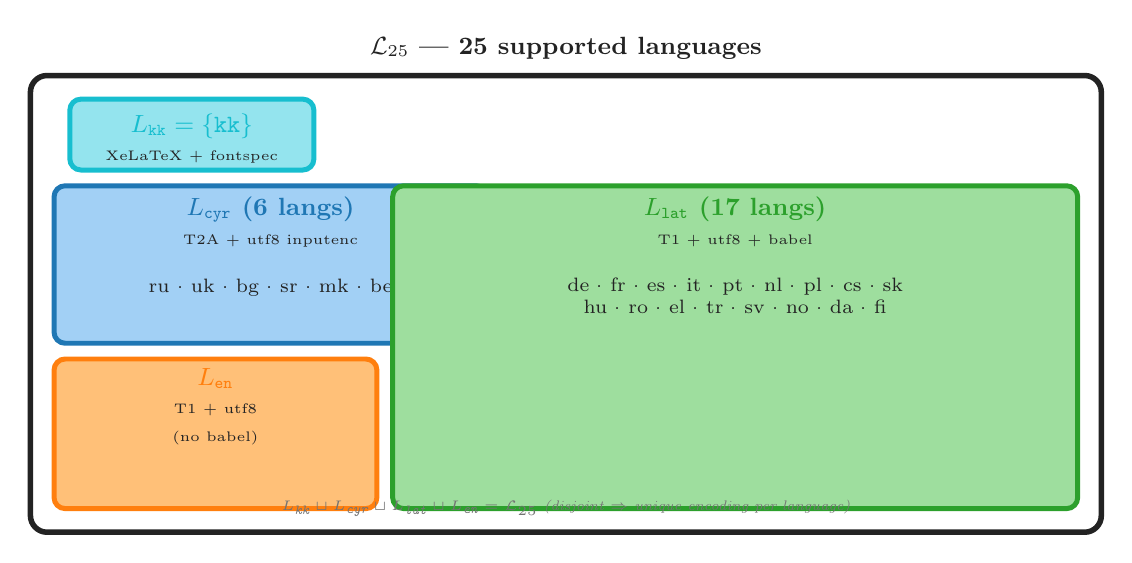
\begin{tikzpicture}
\draw[DG, line width=2pt, rounded corners=6pt]
  (-6.8,-2.9) rectangle (6.8,2.9);
\node[font=\small\bfseries,text=DG] at (0,3.25){$\mathcal{L}_{25}$ — 25 supported languages};

\fill[F6, draw=C6, line width=1.8pt, rounded corners=4pt]
  (-6.3,1.7) rectangle (-3.2,2.6);
\node[font=\small\bfseries,text=C6] at (-4.75,2.25){$L_\texttt{kk}=\{\texttt{kk}\}$};
\node[font=\tiny,text=DG] at (-4.75,1.87){XeLaTeX + fontspec};

\fill[F1, draw=C1, line width=1.8pt, rounded corners=4pt]
  (-6.5,-0.5) rectangle (-1.0,1.5);
\node[font=\small\bfseries,text=C1] at (-3.75,1.2){$L_\texttt{cyr}$ (6 langs)};
\node[font=\tiny,text=DG]           at (-3.75,0.8){T2A + utf8 inputenc};
\node[font=\scriptsize,text=DG]     at (-3.75,0.2){ru · uk · bg · sr · mk · be};

\fill[F3, draw=C3, line width=1.8pt, rounded corners=4pt]
  (-2.2,-2.6) rectangle (6.5,1.5);
\node[font=\small\bfseries,text=C3] at (2.15,1.2){$L_\texttt{lat}$ (17 langs)};
\node[font=\tiny,text=DG]           at (2.15,0.8){T1 + utf8 + babel};
\node[font=\scriptsize,text=DG,align=center,text width=7.5cm]
  at (2.15,0.1) {de · fr · es · it · pt · nl · pl · cs · sk\\
                  hu · ro · el · tr · sv · no · da · fi};

\fill[F2, draw=C2, line width=1.8pt, rounded corners=4pt]
  (-6.5,-2.6) rectangle (-2.4,-0.7);
\node[font=\small\bfseries,text=C2] at (-4.45,-0.95){$L_\texttt{en}$};
\node[font=\tiny,text=DG]           at (-4.45,-1.35){T1 + utf8};
\node[font=\tiny,text=DG]           at (-4.45,-1.7){(no babel)};

\node[font=\tiny\itshape,text=MG] at (0,-2.6)
  {$L_\texttt{kk}\sqcup L_\texttt{cyr}\sqcup L_\texttt{lat}\sqcup
    L_\texttt{en}=\mathcal{L}_{25}$ (disjoint $\Rightarrow$ unique encoding per language)};
\end{tikzpicture}
\caption{Language encoding partition $\mathcal{L}_{25}$ (Definition~9).
         Four disjoint subsets cover all 25 supported languages, each
         mapped to a unique LaTeX encoding stack.}
\label{fig:encoding}
\end{figure}

% ╔══════════════════════════════════════════════════════════════════════════╗
% ║  FIG 17 — TikZ Compile Success Rate by Type Category                   ║
% ╚══════════════════════════════════════════════════════════════════════════╝
\begin{figure}[h!]
\centering
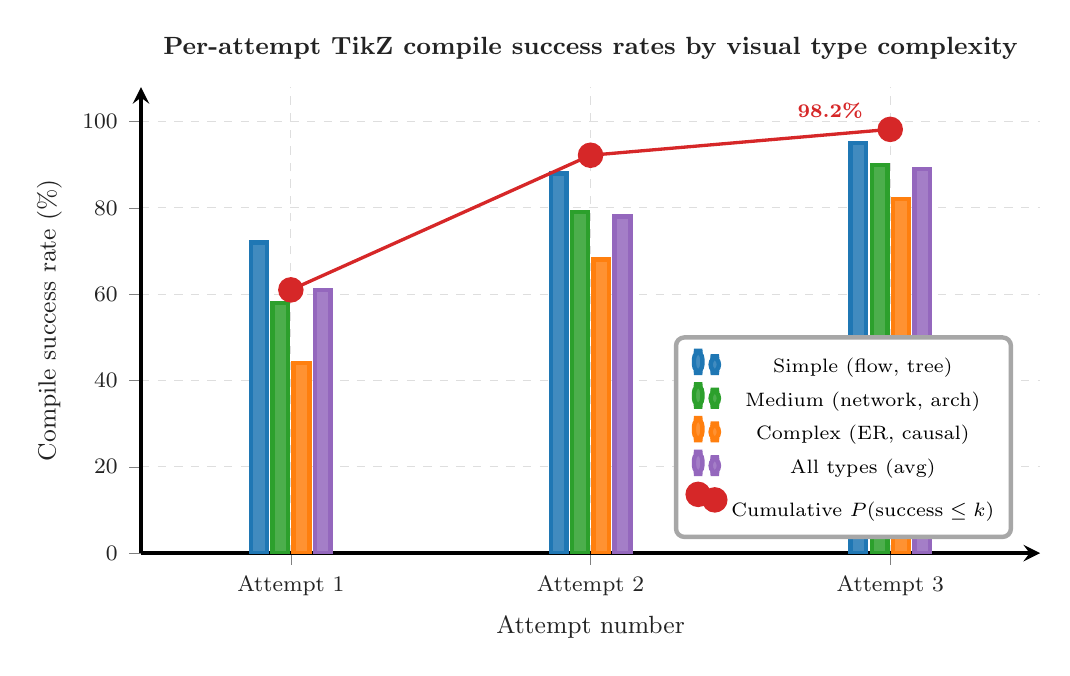
\begin{tikzpicture}
\begin{axis}[PL,
  xlabel={Attempt number},
  ylabel={Compile success rate (\%)},
  title={Per-attempt TikZ compile success rates by visual type complexity},
  xmin=0.5, xmax=3.5, ymin=0, ymax=108,
  xtick={1,2,3},
  xticklabels={Attempt 1,Attempt 2,Attempt 3},
  ytick={0,20,40,60,80,100},
  legend pos=south east,
  ybar, bar width=0.20cm,
]
\addplot[fill=C1!85, draw=C1] coordinates{(1,72)(2,88)(3,95)};
\addlegendentry{Simple (flow, tree)}
\addplot[fill=C3!85, draw=C3] coordinates{(1,58)(2,79)(3,90)};
\addlegendentry{Medium (network, arch)}
\addplot[fill=C2!85, draw=C2] coordinates{(1,44)(2,68)(3,82)};
\addlegendentry{Complex (ER, causal)}
\addplot[fill=C5!85, draw=C5] coordinates{(1,61)(2,78)(3,89)};
\addlegendentry{All types (avg)}
% Cumulative success line
\addplot[C4, very thick, sharp plot, mark=*, mark size=4pt,
         mark options={fill=C4,solid}]
  coordinates{(1,61)(2,92.2)(3,98.2)};
\addlegendentry{Cumulative $P(\text{success}\leq k)$}
\node[font=\scriptsize\bfseries,text=C4,anchor=south] at (axis cs:2.8,98)
  {98.2\%};
\end{axis}
\end{tikzpicture}
\caption{Per-attempt compile success rates by type complexity. The cumulative
         success (red line) exceeds 92\% at $K\!=\!2$ — consistent with
         Theorem~1 at $p\approx0.61$.}
\label{fig:compile-rates}
\end{figure}

% ╔══════════════════════════════════════════════════════════════════════════╗
% ║  FIG 18 — System Invariants Formal Specification                        ║
% ╚══════════════════════════════════════════════════════════════════════════╝
\begin{figure}[h!]
\centering
\begin{tikzpicture}[
  ibox/.style={draw=#1, fill=#2, line width=2pt, rounded corners=4pt,
               text width=13cm, align=left, inner sep=8pt, font=\small}
]
\node[font=\small\bfseries,text=DG] at (0,0.3)
  {Perricheno System Invariants (I1--I5):};

\node[ibox={C1}{L1}] (I1) at (0,-0.4) {%
  \textbf{\color{C1}I1} (Preamble Uniqueness):
  $\forall\,l\in\mathcal{L}_{25},\;\exists!\;P_l:
  \mathtt{buildPreamble}(\mathtt{settings}[l])=P_l$.
  No two languages produce the same preamble string.};

\node[ibox={C3}{L3}, below=0.25cm of I1] (I2) {%
  \textbf{\color{C3}I2} (Citation Safety):
  $\forall\,k\in\mathtt{cite}(\text{mainTex}),\;
  k\in\mathtt{keys}(\text{referencesBib})\;\lor\;k\in\mathtt{stubs}$.
  No \texttt{\textbackslash{}cite} key is unresolved in the output.};

\node[ibox={C2}{L2}, below=0.25cm of I2] (I3) {%
  \textbf{\color{C2}I3} (Billing Monotonicity):
  $\mathcal{B}(T,n)\geq\mathcal{B}(T',n')$ whenever $T\geq T'$ and $n\geq n'$.
  Billed characters are non-decreasing in token count and image count.};

\node[ibox={C5}{L5}, below=0.25cm of I3] (I4) {%
  \textbf{\color{C5}I4} (Order Preservation):
  $\mathtt{concurrentMap}(f,\mathbf{x},N)[i]=f(x_i)$ for all $i\in[1,n]$,
  regardless of worker completion order.};

\node[ibox={C4}{L4}, below=0.25cm of I4] (I5) {%
  \textbf{\color{C4}I5} (Real-Data Guarantee):
  $\forall\,\mathtt{code}\in\mathtt{accepted\_analytics}:\;
  \lnot\,\mathtt{synthetic}(\mathtt{code})$, where
  $\mathtt{synthetic}$ detects
  $\{\mathtt{np.random},\mathtt{rnorm},\mathtt{runif},
  \mathtt{sample},\mathtt{range(N)}\}$
  without column references.};
\end{tikzpicture}
\caption{Five formally stated system invariants. I1--I5 cover uniqueness,
         citation safety, billing monotonicity, order preservation, and
         real-data authenticity — constituting the platform's formal
         correctness specification.}
\label{fig:invariants}
\end{figure}

% ╔══════════════════════════════════════════════════════════════════════════╗
% ║  FIG 19 — Section Length Distributions                                  ║
% ╚══════════════════════════════════════════════════════════════════════════╝
\begin{figure}[h!]
\centering
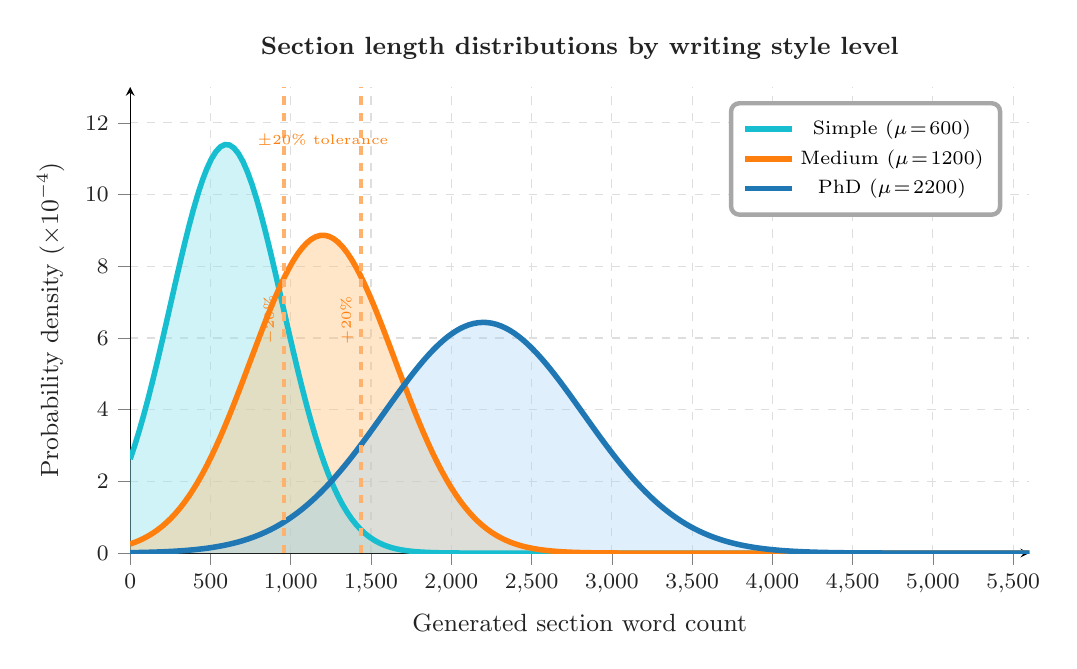
\begin{tikzpicture}
\begin{axis}[PL,
  xlabel={Generated section word count},
  ylabel={Probability density ($\times10^{-4}$)},
  title={Section length distributions by writing style level},
  xmin=0, xmax=5600, ymin=0, ymax=13,
  scaled y ticks=false,
  ytick={0,2,4,6,8,10,12},
  legend pos=north east,
]
% simple ~600 words, sd~350
\addplot[name path=S, C6, line width=2pt, samples=200, domain=0:5600]
  {10000*(1/(350*sqrt(2*3.14159))*exp(-((x-600)^2)/(2*350^2)))};
\addlegendentry{Simple ($\mu\!=\!600$)}
% medium ~1200 words, sd~450
\addplot[name path=M, C2, line width=2pt, samples=200, domain=0:5600]
  {10000*(1/(450*sqrt(2*3.14159))*exp(-((x-1200)^2)/(2*450^2)))};
\addlegendentry{Medium ($\mu\!=\!1200$)}
% phd ~2200 words, sd~620
\addplot[name path=P, C1, line width=2pt, samples=200, domain=0:5600]
  {10000*(1/(620*sqrt(2*3.14159))*exp(-((x-2200)^2)/(2*620^2)))};
\addlegendentry{PhD ($\mu\!=\!2200$)}
% Fill under curves
\addplot[name path=Z, draw=none, domain=0:5600]{0};
\addplot[F6, opacity=0.45] fill between[of=S and Z];
\addplot[F2, opacity=0.40] fill between[of=M and Z];
\addplot[F1, opacity=0.35] fill between[of=P and Z];
% Tolerance bands for medium
\addplot[C2!60, dashed, line width=1.5pt]
  coordinates{(960,0)(960,13)};
\addplot[C2!60, dashed, line width=1.5pt]
  coordinates{(1440,0)(1440,13)};
\node[font=\tiny\bfseries,text=C2,rotate=90,anchor=south]
  at (axis cs:970,6.5){$-20\%$};
\node[font=\tiny\bfseries,text=C2,rotate=90,anchor=south]
  at (axis cs:1450,6.5){$+20\%$};
\node[font=\tiny,text=C2] at (axis cs:1200,11.5){$\pm20\%$ tolerance};
\end{axis}
\end{tikzpicture}
\caption{Modelled section-length distributions for three style levels.
         Shaded fills under each Gaussian show the expected density.
         Dashed lines mark the $\pm20\%$ tolerance enforced around
         the target word count for the medium style.}
\label{fig:distribution}
\end{figure}

% ╔══════════════════════════════════════════════════════════════════════════╗
% ║  FIG 20 — Unified Mathematical System Model $\mathfrak{P}$              ║
% ╚══════════════════════════════════════════════════════════════════════════╝
\begin{figure}[h!]
\centering
\dbox{C1}{L1}{Definition 10}{Perricheno System Model}{%
  The complete system is the tuple
  $\mathfrak{P}=(\mathcal{G},\Gamma,\mathcal{B},\mathcal{M},
  \Phi_\theta,\mathcal{L}_Q,\mathcal{L}_{25},\Pi)$
  — Typed Grammar (Def.\,8), CGRAG Gate (Def.\,2), Billing Op.\ (Def.\,4),
  MDP (Prop.\,2), LCS Operator (Def.\,3), Quality Lattice (Def.\,5),
  Language Partition (Def.\,9), Pipeline Composition (Def.\,1).}

\vspace{0.5em}
\begin{tikzpicture}[
  comp/.style={draw=#1, fill=#2, line width=2pt, rounded corners=5pt,
               minimum width=3.0cm, minimum height=1.05cm,
               align=center, font=\scriptsize\bfseries},
  arr/.style={-{Stealth[length=7pt,width=5pt]}, line width=1.5pt, draw=#1}
]
\node[comp={C1}{F1}]  (Pi)  at (0,   4.2)  {$\Pi$ \\ Pipeline (Def.\,1)};
\node[comp={C2}{F2}]  (G)   at (4.2, 2.1)  {$\mathcal{G}$ \\ Grammar (Def.\,8)};
\node[comp={C5}{F5}]  (Gam) at (4.2,-2.1)  {$\Gamma$ \\ CGRAG (Def.\,2)};
\node[comp={C3}{F3}]  (B)   at (2.1,-4.2)  {$\mathcal{B}$ \\ Billing (Def.\,4)};
\node[comp={C4}{F4}]  (M)   at (-2.1,-4.2) {$\mathcal{M}$ \\ MDP (Prop.\,2)};
\node[comp={C6}{F6}]  (Phi) at (-4.2,-2.1) {$\Phi_\theta$ \\ LCS (Def.\,3)};
\node[comp={C7}{F7}]  (LQ)  at (-4.2, 2.1) {$\mathcal{L}_Q$ \\ Lattice (Def.\,5)};
\node[comp={C8}{L4}]  (L25) at (0,  -0.5)  {$\mathcal{L}_{25}$ \\ Partition (Def.\,9)};

% Central node
\node[draw=C1, fill=F1, line width=2.5pt, circle, minimum size=2.0cm,
      align=center, font=\small\bfseries, text=C1] (sys) at (0,1.1)
  {$\mathfrak{P}$\\System};

% Arrows
\draw[arr={C1}] (Pi) --(sys);
\draw[arr={C2}] (G)  --(sys);
\draw[arr={C5}] (Gam)--(sys);
\draw[arr={C3}] (B)  --(sys);
\draw[arr={C4}] (M)  --(sys);
\draw[arr={C6}] (Phi)--(sys);
\draw[arr={C7}] (LQ) --(sys);
\draw[arr={C4}] (L25)--(sys);

\node[font=\tiny\itshape,text=MG] at (0,-5.8)
  {Tuple $\mathfrak{P}$ constitutes the formal intellectual specification
   of the platform (Definition~10).};
\end{tikzpicture}
\caption{Unified system model $\mathfrak{P}$ (Definition~10) integrating all
         eight formally specified components (Definitions~1--9,
         Propositions~1--2). The tuple uniquely characterises the platform's
         core intellectual contribution for IEEE publication.}
\label{fig:unified}
\end{figure}

\end{document}
